\documentclass[b4paper, landscape, dvipdfmx]{jsarticle}
%----- 必要なパッケージ -----
\usepackage{fancybox,ascmac,otf}
\usepackage{amssymb, amsthm}
\usepackage[leqno]{amsmath}
\usepackage{geometry}
\usepackage{multicol}
\usepackage{tcolorbox}
\usepackage{xcolor}
\usepackage{fancyhdr}
\usepackage{tikz}

% TikZライブラリ
\usetikzlibrary{
    positioning,
    arrows.meta,
    calc,
    shadows,
    shadows.blur,
    intersections,
    angles,
    quotes
}

% tcolorboxライブラリ
\tcbuselibrary{skins, breakable, theorems}

\usepackage{enumitem}
\setlist[enumerate,1]{label=(\arabic*)}
\setlist[itemize]{leftmargin=*}
\newcommand{\ds}{\displaystyle}

%----- レイアウト設定 -----
\geometry{
  left=15mm,
  right=15mm,
  top=20mm,
  bottom=15mm,
  headheight=25pt
}

%----- 数式環境の上下の余白調整 -----
\AtBeginDocument{
  \setlength{\abovedisplayskip}{5pt}
  \setlength{\belowdisplayskip}{5pt}
  \setlength{\abovedisplayshortskip}{0pt}
  \setlength{\belowdisplayshortskip}{3pt}
}

%===========================================================
%  デザイン設定
%===========================================================

%--- 色の定義 ---
\definecolor{printBlue}{RGB}{0, 50, 100}     % 濃紺
\definecolor{printRed}{RGB}{140, 20, 20}     % 濃エンジ
\definecolor{printTeal}{RGB}{0, 60, 60}      % 濃い青緑

%--- 共通スタイル定義 ---
\tcbset{
    chartbox/.style={
        enhanced,
        fonttitle=\sffamily\bfseries,
        boxrule=1pt,
        arc=2pt,
        top=1.0em,
        nobeforeafter,
        enlarge left by=-2mm,
        enlarge right by=-2mm,
        drop fuzzy shadow,
        colback=white,
        attach boxed title to top left={xshift=10pt, yshift*=-\tcboxedtitleheight/2},
        boxed title style={frame hidden, sharp corners, rounded corners=southeast, arc=3pt}
    }
}

%--- 各種ボックス環境定義 ---
\newtcolorbox{any}[1]{
    enlarge left by=0mm, enlarge right by=0mm,
    enhanced, frame hidden, colback=white, title={#1},
    attach boxed title to top left={xshift=0mm, yshift=0mm},
    coltitle=white, fonttitle=\bfseries\sffamily,
    boxed title style={
        colback=black!80, frame hidden, arc=4pt, outer arc=4pt,
        sharp corners=south, boxrule=0pt,
        top=1mm, bottom=1mm, left=3mm, right=3mm
    },
    underlay boxed title={
        \draw[thick, black!80] (title.south west) -- (title.south west-|frame.east);
    },
    breakable, top=5mm, left=2mm, right=2mm, bottom=0mm,
    before skip=1em, after skip=1em,
    segmentation style={draw=black!40, dashed}
}

\newtcolorbox{eg}[1]{
    chartbox,
    colframe=printBlue,
    coltitle=white,
    title=\textbf{例題 #1},
    boxed title style={colback=printBlue},
    segmentation style={draw=printBlue, line width=0.5pt, dashed}
}

\newtcolorbox{prac}[1]{
    chartbox,
    colframe=printRed,
    coltitle=white,
    title=\textbf{練習 #1},
    boxed title style={colback=printRed}
}

\newtcolorbox{thm}[1]{
    chartbox,
    colframe=printTeal,
    coltitle=white,
    title=\textbf{#1},
    boxed title style={colback=printTeal}
}

\newtcolorbox{answer}[1][height fill]{
    enhanced,
    title={Memo / Answer},
    colframe=black!80,
    colback=white,
    coltitle=black!60,
    fonttitle=\sffamily\bfseries,
    attach boxed title to top left={xshift=5mm, yshift*=-\tcboxedtitleheight/2},
    boxed title style={frame hidden, colback=white},
    boxrule=1pt,
    arc=1pt,
    nobeforeafter,
    enlarge left by=-2mm, 
    enlarge right by=-2mm, 
    height fill,
    segmentation style={draw=black!20, solid},
    underlay={
        \begin{tcbclipinterior}
            \draw[step=5mm, black!5, ultra thin] (interior.south west) grid (interior.north east);
        \end{tcbclipinterior}
    }, 
    #1
}

%----- ヘッダーの設定 -----
\pagestyle{fancy}
\fancyhf{}
\fancyhead[C]{%
    \begin{tikzpicture}[remember picture, overlay]
        \node[anchor=north west, fill=printBlue, minimum width=\paperwidth, minimum height=5pt] at (current page.north west) {};
    \end{tikzpicture}
}
\fancyhead[L]{\small \textcolor{black!90}{数学C $>$ 第1章--平面ベクトル $>$ 第8回 \textbf{3点が一直線上にある条件}}}
\fancyhead[R]{\small 年 \hspace{1cm} 組 \hspace{1cm} 番 \quad 氏名 \hspace{6cm}}
\renewcommand{\headrulewidth}{0pt}

\begin{document}

%=============================================================================
% 1枚目:共線条件の基本
%=============================================================================
\begin{multicols}{2}

%-----------------------------------------------------------------------------
% 左カラム:基本定理
%-----------------------------------------------------------------------------
\begin{any}{1. 「一直線上にある」を式にする}
    ベクトルの強みは, 「3点が一直線上にある(共線)」という幾何学的な状態を, シンプルな等式で表現できる点にある.

    \begin{thm}{共線条件 (基本形)}
        2点 A, B が異なるとき, 点 P が直線 AB 上にあるための必要十分条件は,
        \[ \overrightarrow{\text{AP}} = k \overrightarrow{\text{AB}} \]
        となる実数 $k$ が存在することである.
    \end{thm}
    
    \begin{center}
    \begin{tikzpicture}[scale=1.0, >=stealth]
        \draw[thick, gray!50] (-1,0) -- (5,0);
        \fill (0,0) circle (2pt) node[below] {A};
        \fill (3,0) circle (2pt) node[below] {B};
        \fill (4.5,0) circle (2pt) node[below] {P};
        
        \draw[->, thick, printBlue] (0,0) -- (3,0) node[midway, above] {$\vec{u}$};
        \draw[->, very thick, printRed, dashed] (0,0) -- (4.5,0);
        \node[above, printRed] at (2.25, 0.5) {$\vec{u}$ の $k$ 倍};
        
        \node[align=left, scale=0.9] at (2, -1) {向きが同じ(または逆)で\\びよーんと伸ばせば一致する $\to$ 実数倍};
    \end{tikzpicture}
    \end{center}
    
    これは「平行条件 $\vec{a} // \vec{b} \iff \vec{b}=k\vec{a}$」において, 始点を A に共有させたものと同じである.
\end{any}

%-----------------------------------------------------------------------------
% 右カラム:位置ベクトルでの表現
%-----------------------------------------------------------------------------
\columnbreak

\begin{any}{2. 位置ベクトルと係数の和}
    始点を任意の点 O(原点)とした場合どうなるか.
    $\overrightarrow{\text{AP}} = k \overrightarrow{\text{AB}}$ を書き換えてみる.
    \begin{align*}
        \vec{p} - \vec{a} &= k(\vec{b} - \vec{a}) \\
        \vec{p} &= (1-k)\vec{a} + k\vec{b}
    \end{align*}
    ここで $1-k=s, k=t$ とおくと, $s+t=1$ となる.

    \begin{thm}{共線条件 (係数の和が1)}
        点 P が直線 AB 上にある $\iff$
        \[ \vec{p} = s\vec{a} + t\vec{b} \quad \text{かつ} \quad s+t=1 \]
    \end{thm}

    \begin{eg}{1 (基本確認)}
        $\triangle$OAB において, 
        $\overrightarrow{\text{OP}} = \frac{1}{3}\vec{a} + \frac{2}{3}\vec{b}$ とする.
        点 P は直線 AB 上にあるか確認せよ.
        \tcblower
        \textbf{解答:} 
        係数の和を確認する.
        $\frac{1}{3} + \frac{2}{3} = 1$.
        よって, 点 P は直線 AB 上にある.
        (具体的には $2:1$ に内分する点)
        \vspace{2cm}
    \end{eg}
\end{any}

\end{multicols}

%=============================================================================
% 2枚目:応用(証明問題・図形の性質)
%=============================================================================
\newpage
\begin{multicols}{2}

%-----------------------------------------------------------------------------
% 左カラム:一直線上にあることの証明
%-----------------------------------------------------------------------------
\begin{any}{3. 図形の証明問題}
    「3点 A, B, C が一直線上にあることを示せ」と言われたら, 
    \[ \overrightarrow{\text{AC}} = k \overrightarrow{\text{AB}} \]
    となる実数 $k$ を見つければよい(始点はどこでもよい).

    \begin{eg}{2 三角形と共線条件}
        $\triangle$OAB において, $\vec{a}=\overrightarrow{\text{OA}}, \vec{b}=\overrightarrow{\text{OB}}$ とする.
        $\overrightarrow{\text{OP}} = 3\vec{a} - 2\vec{b}$, $\overrightarrow{\text{OQ}} = -\frac{3}{2}\vec{a} + \vec{b}$.
        このとき, O, P, Q は一直線上にあることを示せ.
        \tcblower
        \vspace{8cm}
    \end{eg}
\end{any}

%-----------------------------------------------------------------------------
% 右カラム:係数和=1の威力
%-----------------------------------------------------------------------------
\columnbreak

\begin{any}{4. 「係数の和が1」の応用}
    $\overrightarrow{\text{OP}} = s\vec{a} + t\vec{b}$ において,
    点 P が直線 AB 上にある条件は $s+t=1$ である.
    これを利用して, 未知の係数を決定することができる.

    \begin{eg}{3 (交点の位置ベクトル・導入)}
        $\triangle$OAB において, 辺 OA を $1:2$ に内分する点を C, 辺 OB を $2:3$ に内分する点を D とする.
        線分 AD と BC の交点を P とする.
        $\overrightarrow{\text{OA}}=\vec{a}, \overrightarrow{\text{OB}}=\vec{b}$ とする.
        
        (1) 点 P は直線 AD 上にあるので, $\overrightarrow{\text{OP}} = (1-s)\vec{a} + s\overrightarrow{\text{OD}}$ と表せる. これを $\vec{a}, \vec{b}$ で表せ.
        
        (2) 点 P は直線 BC 上にあるので, $\overrightarrow{\text{OP}} = (1-t)\overrightarrow{\text{OC}} + t\vec{b}$ と表せる. これを $\vec{a}, \vec{b}$ で表せ.
        
        (3) $\vec{a}, \vec{b}$ の一次独立性を用いて $s, t$ を求め, $\overrightarrow{\text{OP}}$ を決定せよ.
        
        \tcblower
        \vspace{6cm}
    \end{eg}
    \begin{tcolorbox}[colback=yellow!10, frame hidden, title={次回予告}]
        この「2通りで表して係数比較」が, ベクトルにおける交点計算の必勝パターンである.
    \end{tcolorbox}
\end{any}

\end{multicols}

%=============================================================================
% 3枚目:確認テスト(問題)
%=============================================================================
\newpage
\fancyhead[L]{\small \textcolor{black!90}{数学C $>$ 第1章--平面ベクトル $>$ 第8回--\textbf{確認テスト}}}
\begin{multicols}{2}

\begin{any}{確認テスト (A: 基本)}
    \begin{prac}{A1 (一直線上にある条件)}
        平行四辺形 ABCD において, 辺 BC の中点を E, 辺 CD の中点を F とする.
        $\overrightarrow{\text{AB}}=\vec{b}, \overrightarrow{\text{AD}}=\vec{d}$ とする.
        $\overrightarrow{\text{AE}}, \overrightarrow{\text{AF}}$ を $\vec{b}, \vec{d}$ で表し, 
        $\overrightarrow{\text{AC}}$ との間に共線関係があるか(一直線上にあるか)調べよ.
        \vspace{1em}
        \begin{center}
        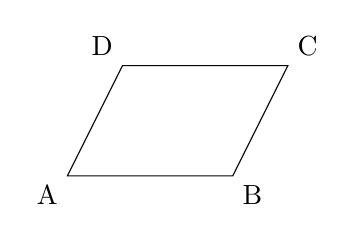
\begin{tikzpicture}[scale=0.7]
            \draw (0,0) node[below left]{A} -- (3,0) node[below right]{B} -- (4,2) node[above right]{C} -- (1,2) node[above left]{D} -- cycle;
        \end{tikzpicture}
        \end{center}
    \end{prac}
    \begin{answer}[height=5cm]
    \end{answer}

    \begin{prac}{A2 (係数の和)}
        $\triangle$ABC と点 P について, 
        \[ \overrightarrow{\text{AP}} = \frac{1}{4}\overrightarrow{\text{AB}} + k \overrightarrow{\text{AC}} \]
        が成り立つ. 点 P が直線 BC 上にあるとき, 実数 $k$ の値を求めよ.
    \end{prac}
    \begin{answer}[height=5cm]
    \end{answer}
\end{any}

\columnbreak

\begin{any}{確認テスト (B: 標準)}
    \begin{prac}{B1 (一直線の証明)}
        $\triangle$OAB において, $\overrightarrow{\text{OA}}=\vec{a}, \overrightarrow{\text{OB}}=\vec{b}$ とする.
        辺 OA を $3:2$ に内分する点を C, 辺 OB を $3:1$ に内分する点を D とする.
        線分 BC と AD の交点を P とするとき, $\overrightarrow{\text{OP}}$ を $\vec{a}, \vec{b}$ で表せ.
        
        (ヒント: PはBC上 $\to \vec{p} = (1-s)\vec{b} + s\vec{c}$ ... )
    \end{prac}
    \begin{answer}[height=12cm]
    \end{answer}
\end{any}

\end{multicols}

%=============================================================================
% 4枚目:確認テスト(解答)
%=============================================================================
\newpage
\fancyhead[L]{\small \textcolor{black!90}{数学C $>$ 第1章--平面ベクトル $>$ 第8回 \textbf{【解答解説】}}}

\begin{multicols}{2}

\begin{any}{解答 (A: 基本)}
    \begin{answer}[height=12cm]
    \color{printRed}
    \textbf{A1 解答}:\\
    (1) $\overrightarrow{\text{AE}}$: EはBCの中点なので $\overrightarrow{\text{BE}}=\frac{1}{2}\vec{d}$.
        \[ \overrightarrow{\text{AE}} = \vec{b} + \frac{1}{2}\vec{d} \]
        (2) $\overrightarrow{\text{AF}}$: FはCDの中点なので $\overrightarrow{\text{DF}}=\frac{1}{2}\vec{b}$.
        \[ \overrightarrow{\text{AF}} = \vec{d} + \frac{1}{2}\vec{b} \]
        (3) $\overrightarrow{\text{AC}} = \vec{b} + \vec{d}$.
        
        $\overrightarrow{\text{AE}} + \overrightarrow{\text{AF}} = \frac{3}{2}(\vec{b}+\vec{d}) = \frac{3}{2}\overrightarrow{\text{AC}}$.
        これは A, E, F が一直線という意味ではない.
        $\overrightarrow{\text{AC}} = k \overrightarrow{\text{AE}}$ となる $k$ は存在しないため, A, C, E は一直線上にはない. (図を見れば明らか)
    \textbf{補足:} 問題の意図としては「計算練習」です.
    もし A, E, F が一直線上にあるなら $\overrightarrow{\text{AF}} = k \overrightarrow{\text{AE}}$ となるはずですが,
    $\vec{d} + \frac{1}{2}\vec{b} = k(\vec{b} + \frac{1}{2}\vec{d})$
    係数比較すると $1 = k/2, 1/2 = k \implies k=2, k=1/2$ (矛盾).
    よって一直線上にはありません.
    \end{answer}

    \begin{answer}[height=5cm]
    \color{printRed}
    \textbf{A2 解答:} \\
    点 P が直線 BC 上にある条件は, $\overrightarrow{\text{AB}}$ と $\overrightarrow{\text{AC}}$ の係数の和が 1 になることである.
    (始点 A が基準になっているため)
    
    \[ \frac{1}{4} + k = 1 \]
    \[ \therefore \quad k = \frac{3}{4} \]
    
    \textbf{確認:} $\vec{p} = \frac{1}{4}\vec{b} + \frac{3}{4}\vec{c} = \frac{1\vec{b} + 3\vec{c}}{4}$.
    これは線分 BC を $3:1$ に内分する点である.
    \end{answer}
\end{any}

\columnbreak

\begin{any}{解答 (B: 標準)}
    \begin{answer}[height fill]
    \color{printRed}
    \textbf{B1 解答:} \\
    条件より $\overrightarrow{\text{OC}} = \frac{3}{5}\vec{a}, \quad \overrightarrow{\text{OD}} = \frac{3}{4}\vec{b}$.
    
    (1) 点 P は線分 BC 上にあるので, $s : (1-s)$ に内分すると考える.
    \[ \overrightarrow{\text{OP}} = (1-s)\overrightarrow{\text{OB}} + s\overrightarrow{\text{OC}} = (1-s)\vec{b} + \frac{3}{5}s\vec{a} \quad \cdots (1) \]
    
    (2) 点 P は線分 AD 上にあるので, $t : (1-t)$ に内分すると考える.
    \[ \overrightarrow{\text{OP}} = (1-t)\overrightarrow{\text{OA}} + t\overrightarrow{\text{OD}} = (1-t)\vec{a} + \frac{3}{4}t\vec{b} \quad \cdots (2) \]
    
    (3) 係数比較
    $\vec{a}, \vec{b}$ は一次独立なので:
    \[
    \begin{cases}
        \frac{3}{5}s = 1-t \\
        1-s = \frac{3}{4}t
    \end{cases}
    \]
    第2式より $s = 1 - \frac{3}{4}t$. これを第1式へ代入.
    $\frac{3}{5}(1-\frac{3}{4}t) = 1-t$ \\
    $12(1-\frac{3}{4}t) = 20(1-t)$ (両辺20倍) \\
    $12 - 9t = 20 - 20t \implies 11t = 8 \implies t = \frac{8}{11}$.
    
    (2)へ代入して:
    $\overrightarrow{\text{OP}} = (1-\frac{8}{11})\vec{a} + \frac{3}{4}\cdot\frac{8}{11}\vec{b} = \frac{3}{11}\vec{a} + \frac{6}{11}\vec{b}$
    
    \textbf{答え:} $\boldsymbol{\overrightarrow{\text{OP}} = \frac{3}{11}\vec{a} + \frac{6}{11}\vec{b}}$
    \end{answer}
\end{any}

\end{multicols}
\end{document}